\documentclass{article}
\usepackage{tikz}
\usetikzlibrary{shapes.geometric, arrows}

\begin{document}

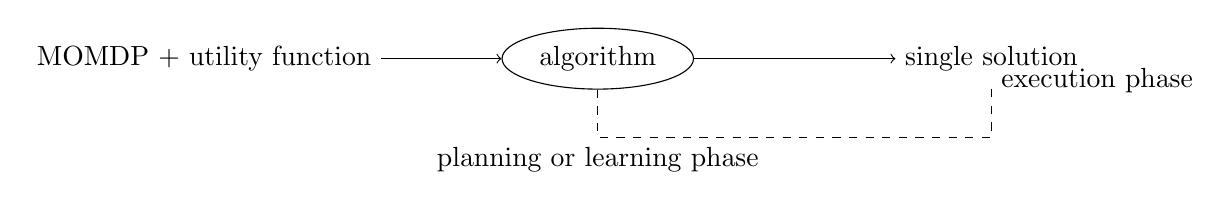
\begin{tikzpicture}[node distance=2cm]
    \node (start) [draw, ellipse] {algorithm};
    \node (input) [left of=start, xshift=-3cm] {MOMDP + utility function};
    \node (output) [right of=start, xshift=3cm] {single solution};
    
    \draw[->] (input) -- (start);
    \draw[->] (start) -- (output);
    
    \draw[dashed] (start) -- ++(0,-1) node[below] {planning or learning phase};
    \draw[dashed] (start) -- ++(0,-1) -| (output) node[below right] {execution phase};
\end{tikzpicture}

\end{document}